\chapter{Objetivos}
\label{cap:capitulo3}

\begin{flushright}
\begin{minipage}[]{10cm}
\emph{Establecer metas es el primer paso para convertir lo invisible en visible.}\\
\end{minipage}\\

Tony Robbins\\
\end{flushright}

\vspace{1cm}
\setcounter{footnote}{18} 

Tras haber establecido el marco contextual del presente proyecto, se procede a presentar la descripción del problema, los requisitos, las competencias tanto adquiridas como empleadas, la metodología y el plan de trabajo seguido.

\section{Descripción del problema}
\label{sec:descripcion}

La idea de este trabajo fin de grado nace tras los acontecimientos vividos por la \ac{DANA} que afectó a la zona de Toledo y Madrid el pasado septiembre de 2023. Estos hechos dejaron inundaciones, pueblos anegados, carreteras cortadas, muchos vecinos perdieron sus casas, y desgraciadamente se cobró la vida de tres personas. 

%% Mejorar esta parte por que se da a entender que la dana fue culpa de las carreteras
%Esta situación se produjo, en parte, por la falta de mantenimiento de los pavimentos y carreteras y que posteriormente a lo sucedido, también fue una de las infraestructuras que más tardaron en arreglarse. La principal causa de que eso ocurriese es los bajos recursos y la falta de mano de obra que justamente hay en la zona que sucedieron los hechos. Los operarios que conforman esta mano de obra llevan tiempo exigiendo mejoras de seguridad en su entorno laboral como defiende la Plataforma de Trabajadores de Conservación de Carreteras\footnote{\url{https://conservacion.es/index.php?option=com_content&view=article&id=1&Itemid=101}}.  
Tras lo sucedido, las carreteras fueron las infraestructuras que más tardaron en arreglarse. La principal causa de que eso ocurriese es la falta de fondos, lo que conlleva un escaso mantenimiento. Además, los operarios que conforman la mano de obra llevan tiempo exigiendo mejoras de seguridad en su entorno laboral, como defiende la Plataforma de Trabajadores de Conservación de Carreteras\footnote{\url{https://conservacion.es/index.php?option=com_content&view=article&id=1&Itemid=101}}.
   
La solución propuesta en este trabajo busca ayudar a mejorar esta situación, proporcionando un robot de bajo coste y accesible para cualquier persona y que sirva para poder mejorar el mantenimiento de las carreteras y reducir el riesgo de exposición de los operarios. Por lo tanto, este proyecto pretende, como objetivo principal, crear un robot que, usando materiales de bajo coste, sea capaz de navegar por las carreteras, detectar los baches que vaya encontrando y sea capaz de estimar el área del bache para hacer una estimación media del volumen que ocupa dicho bache y poder ser tapado. De igual manera, todo quedará registrado en una interfaz web en la que cada bache quedará marcado sobre un mapa con su correspondiente descripción para que los operarios puedan operar cuando estimen oportuno.

Con el fin de alcanzar este objetivo principal, se han establecido los siguientes subobjetivos:

\begin{enumerate}
	\item{} Investigar los robots o soluciones actuales que cumplan con las características y objetivos establecidos.
	\item{} Seleccionar los componentes \textit{hardware} de bajo coste necesarios para construir el esqueleto del robot.
	\item{} Analizar las diferentes opciones de diseño que más encajen con la forma del robot.
	\item{} Diseñar las piezas en CAD usando herramientas de \textit{software} libre.
	\item{} Usar material típico de impresión 3D para imprimir las partes del robot, como puede ser ABS o PLA. 
	\item{} Desarrollar un modelo del robot para que pueda ser usado en simulación usando herramientas robóticas. 
	\item{} Desarrollar software necesario usando herramientas robóticas para poder controlar el robot físico. 
	\item{} Realizar algunos experimentos en entornos reales o adaptados.  
\end{enumerate}
 

\section{Requisitos}
\label{sec:requisitos}

Tras nombrar los objetivos y subobjetivos a cumplir en este proyecto, se enumeran los requisitos que se han de satisfacer: 

\begin{enumerate}
	\item{} El coste total de la fabricación del robot no debe superar los 250€.
	\item{} Todas las piezas diseñadas deben poderse imprimir en cualquiera impresora convencional.
	\item{} Se usará Ubuntu con soporte a largo plazo como sistema operativo, tanto para el ordenador como para el robot.
	\item{} A fin de facilitar la implementación de este proyecto para cualquier tipo de usuario, no será necesario disponer de ninguna tarjeta gráfica de uso dedicado para entrenar los modelos. 
	\item{} Los modelos entrenados se deben ajustar a las limitaciones hardware del robot.
	\item{} Se busca que sea un proyecto a largo plazo, por eso se debe realizar la integración con la plataforma ROS 2. 
\end{enumerate}

\section{Competencias}
\label{sec:competencias}

A continuación se detallan las competencias que se han empleado y adquirido para la realización del presente trabajo fin de grado.
   
\subsection{Competencias empleadas}
\label{subsec:competenciase}
Las competencias empleadas para la realización de este proyecto, y que han sido tomadas de las distintas asignaturas del grado, son las siguientes: 

\begin{enumerate}
	\item{Evolución y futuro de la robótica: \textit{CE1.} Capacidad para analizar la evolución de la Ingeniería Robótica y ser capaz de identificar sus aplicaciones, oportunidades de emprendimiento y su impacto en el futuro. 
	Esta competencia ha sido empleada para poder desarrollar los Capítulos 1 y 2 de este proyecto.}
	\item{Laboratorio de sistemas: \textit{CE9.} Capacidad de conocer y manejar los sistemas y las herramientas de las que dispone para su gestión y programación. 
	Esta competencia ha sido empleada para poder configurar y ejecutar código del robot en entornos no gráficos.}
	\item{Sensores y actuadores: \textit{CE12.} Capacidad de diseñar robots y sistemas inteligentes atendiendo a los elementos de sensorización y actuación más adecuados dependiendo de la aplicación, los requerimientos del sistema y las condiciones del entorno. 
	Esta competencia ha sido empleada para poder encontrar los componentes \textit{hardware} necesarios para poder llevar a cabo el esqueleto del robot.}
	\item{Arquitectura \textit{software} para robots: \textit{CE15.} Capacidad de diseñar y programar aplicaciones robóticas y sistemas inteligentes en red usando \textit{middlewares}, mecanismos de comunicación y estándares propios del ámbito de la Ingeniería Robótica. 
	Esta competencia ha sido empleada en el momento de decidir el tipo de arquitectura \textit{software} necesaria a implementar en el robot.}
	\item{Visión artificial: \textit{CE25.} Capacidad de conocer y aplicar métodos de extracción de información a partir de la información percibida por cámaras y sensores 3D al desarrollo de aplicaciones en robots y sistemas inteligentes. 
	Esta competencia ha sido empleada para poder extraer información de la cámara y ser capaz de tratarla.}
	\item{Mecatrónica: \textit{CE32.} Capacidad de diseñar y construir robots móviles. Esta competencia ha sido empleada en el diseño e impresión en 3D del robot.}
	\item{Aprendizaje automático: \textit{CE27.} Capacidad de construir sistemas capaces de resolver problemas a partir de información no estructurada proporcionada por ejemplos o por la experiencia. 
	Esta competencia ha sido empleada para poder ser capaz de crear modelos de aprendizaje automático y aplicarlos al robot.}
\end{enumerate}

\subsection{Competencias adquiridas}
\label{subsec:competenciasa}

Las competencias adquiridas con el desarrollo de este trabajo fin de grado, y que aparecen descritas en la guía docente de la propia asignatura, son las siguientes: 

\begin{enumerate}
	\item{\textit{CB2.} Que los estudiantes sepan aplicar sus conocimientos a su trabajo o vocación de una forma profesional y posean las competencias que suelen demostrarse por medio de la elaboración y defensa de argumentos y la resolución de problemas dentro de su área de estudio. 
	Esta competencia se adquiere gracias a la aplicación de las competencias empleadas justificadas anteriormente y que se pueden ver plasmadas en todo el proyecto.}
	\item{\textit{CB4.} Que los estudiantes puedan transmitir información, ideas, problemas y soluciones a un público tanto especializado como no especializado. 
	Esta competencia se adquiere al describir de forma precisa y comprensible todo el proceso complejo implicado en este proyecto dentro del presente documento.}
	\item{\textit{CB5.} Que los estudiantes hayan desarrollado aquellas habilidades de aprendizaje necesarias para emprender estudios posteriores con un alto grado de autonomía. 
	Esta competencia se logra al adquirir el conocimiento suficiente para desarrollar este trabajo de forma totalmente autónoma, contrastando información con distintas fuentes, haciendo pruebas con distintos tipos de \textit{software}, entre otras.}
	\item{\textit{CE28.} Desarrollo de las capacidades adecuadas para realizar un ejercicio original individual (o excepcionalmente colectivo), presentarlo y defenderlo ante un tribunal universitario, consistente en un proyecto en el ámbito de las tecnologías específicas del campo de la Robótica de naturaleza profesional en el que se sinteticen e integren las competencias adquiridas en las enseñanzas.
	Esta última competencia se cumple con el desarrollo de este proyecto: que abarca desde la elección del tema, el conocer el estado del arte, la implementación tanto \textit{hardware} como \textit{software}, el desarrollo de la presente memoria hasta su defensa ante un tribunal.}
\end{enumerate}


\section{Metodología}
\label{sec:metodologia}

Para llevar a cabo este proyecto se ha optado por seguir una metodología que se iniciaba con una profunda investigación sobre el estado del arte para comprobar la viabilidad del desarrollo del presente proyecto. Posteriormente, tras haber elegido el \textit{hardware} necesario para el robot, se decidió usar una metodología experimental que ayudó a decidir el diseño final que tendría el robot. Una vez cumplido esto, se imprimieron y ensamblaron las distintas piezas. 


Para dar soporte \textit{software} al robot real se probó y configuró cada sensor y actuador del robot en distintos sistemas operativos y versiones hasta encontrar la combinación que mejor cumpliese todos los objetivos. Una vez conseguido eso, se decidió seguir un ciclo de desarrollo conocido como \ac{PDCA} y así poder ir haciendo pequeños avances consistentes hasta llegar a una versión completamente funcional. Para el desarrollo del robot simulado también se decidió usar la metodología \acs{PDCA}. Esta metodología sigue los siguientes pasos cíclicos descritos en la Figura \ref{fig:PDCA}. 

%\begin{enumerate}
%	\item{\textit{Planear}}. Ante el problema presentado, se decide qué hacer.
	
%	\item{\textit{Hacer}}. Tras conocer qué hacer, se pone en marcha lo planeado previamente.
	
%	\item{\textit{Comprobar}}. Tras conocer los resultados obtenidos, se comprueban.
	
%	\item{\textit{Actuar}}. Tras comprobar los resultados, se ajusta lo que tiene que ser corregido. 

%\end{enumerate}

\begin{figure} [h!]
	\begin{center}
			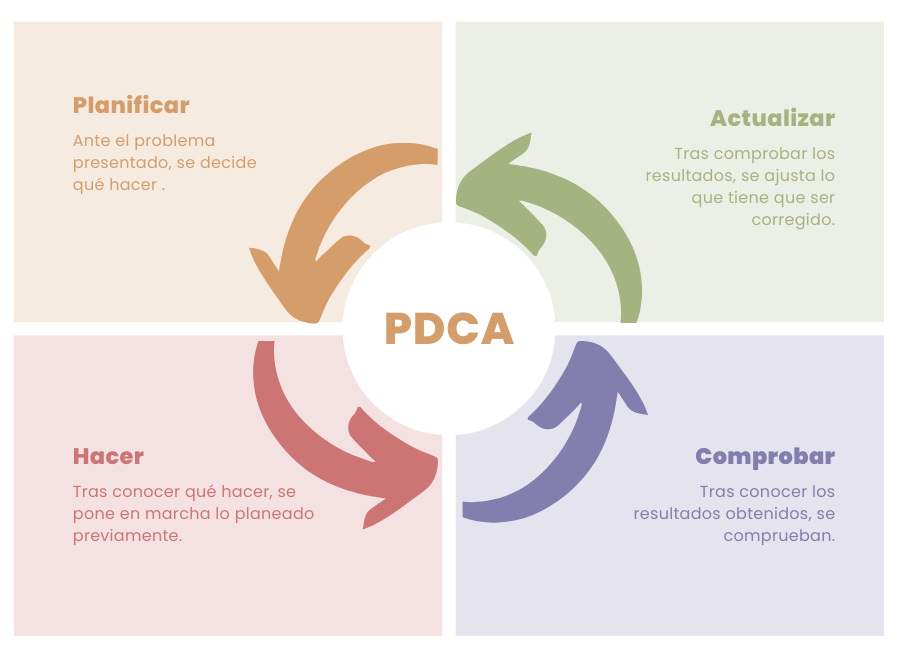
\includegraphics[width=15cm]{figs/PDCA.png}
		\end{center}
	\caption{Método PDCA} 
\label{fig:PDCA}
\end{figure}


\section{Plan de trabajo}
\label{sec:plantrabajo}

El desarrollo del presente trabajo fin de grado se ha dividido en las siguientes etapas: 

\begin{enumerate}
	\item{\textit{Investigación del estado del arte}}. En esta fase inicial, se realizaron búsquedas en plataformas online como Google Scholar\footnote{\url{https://scholar.google.es/}}, Web of Science del FECYT\footnote{\url{https://www.webofscience.com/wos/alldb/basic-search}} que está basa en Web of Science de Clarivate\footnote{\url{https://clarivate.com/products/scientific-and-academic-research/research-discovery-and-workflow-solutions/webofscience-platform/}}, y otras relacionadas con el mantenimiento de carreteras con el fin de encontrar soluciones al problema descrito. 
	
	\item{\textit{Planteamiento hardware del robot}}. Una vez conocida la viabilidad del proyecto, se decidió estudiar qué componentes \textit{low-cost} eran necesarios para dar forma al esqueleto del robot. 
	
	\item{\textit{Diseño de prototipos del robot}}. Tras conocer cuál será el esqueleto del robot, usando cartón y pegamento se hicieron una serie de prototipos hasta encontrar la solución final. Posteriormente se usó la herramienta FreeCAD para modelar las distintas piezas.
	
	\item{\textit{Impresión 3D y ensamblaje de las piezas}}. Una vez el diseño estaba hecho, se decidió imprimirlo usando filamento de tipo PLA azul. Finalmente, se produjo el ensamblaje de todas las piezas.
	
	\item{\textit{Desarrollo del robot en simulación}}. Tras tener el robot completamente montado, se decidió desarrollar el modelo del robot pero esta vez para que se pudiera trabajar con él en simulación; en este caso, usando Gazebo.
	
	\item{\textit{Configuración hardware del robot}}. Tras tener al robot listo en simulación, se decidió configurar cada componente \textit{hardware} del robot en distintos sistemas operativos hasta encontrar el que mejor encajase con la arquitectura del mismo. 
	
	\item{\textit{Desarrollo software del robot en físico}}. Una vez el robot está completamente configurado y listo para operar en un entorno real, se desarrollaron una serie de nodos en ROS 2. Estos ayudan al correcto funcionamiento de cada componente hardware siguiendo el propósito buscado. 
	
	\item{\textit{Experimentos y aplicaciones del robot}}. En esta etapa final, se realizaron distintos experimentos de cada componente, así como se proporcionó dos posibles aplicaciones completas del robot que permitían demostrar que se cumplía el objetivo principal.

\end{enumerate}

Asimismo, a lo largo de todo el proceso se ha ido elaborando la presente memoria. La dinámica seguida con el tutor ha sido de reuniones semanales o cada dos semanas, dependiendo de la disponibilidad por las dos partes. En dichas reuniones se comentaban todos los avances realizados y se proponían aspectos a mejorar, sugerencias, y se definían nuevos objetivos a conseguir. 

Todo el contenido del proyecto está alojado en un repositorio público de GitHub\footnote{\url{https://github.com/RoboticsURJC/tfg-jlopez}}. Además, todo el trabajo diario está documentado en el apartado Wiki\footnote{\url{https://github.com/RoboticsURJC/tfg-jlopez/wiki}} de dicho repositorio; dividido en \textit{diario} y en \textit{evolución del proyecto}. El apartado de \textit{diario} trata de contar de forma coloquial qué se ha ido realizando cada día o cada pocos días. Por otro lado, en \textit{evolución del proyecto} se puede encontrar la explicación detallada de ciertos códigos, así como de conceptos teóricos, entre otros detalles.\\\\\\ % 3 saltos de línea

Tras conocer todos los objetivos, subobjetivos, requisitos, competencias, metodología y plan de trabajo llevado a cabo para la realización de este proyecto, se procede a tratar las plataformas de desarrollo usadas. 



